\documentclass[tikz,border=5pt]{standalone}
\usepackage[utf8]{inputenc}
\usepackage{tikz}
\usetikzlibrary{shapes.geometric, arrows.meta, positioning, shadows.blur, calc, fit, backgrounds}

% --- Professional Colors ---
\definecolor{noiseRed}{RGB}{214, 69, 65}        % OCR Noise (Input Error)
\definecolor{groundBlue}{RGB}{64, 112, 175}     % Grounding (Processing)
\definecolor{mismatchOrange}{RGB}{230, 126, 34} % Vision-Lang Mismatch
\definecolor{outputPurple}{RGB}{142, 68, 173}   % Final Incorrect Output

% --- Global Style Definitions (Prevents Compile Errors) ---
\tikzset{
    % Base Block Style
    process/.style={
        rectangle, 
        rounded corners=2mm, 
        minimum width=3.8cm,      
        minimum height=1.0cm,     
        text centered, 
        text width=3.5cm,         
        font=\sffamily\footnotesize, 
        draw=gray!40,
        thick,
        blur shadow={shadow blur steps=3}
    },
    % Specific Role Styles
    stepNoise/.style={process, fill=noiseRed!10, draw=noiseRed!80!black},
    stepGround/.style={process, fill=groundBlue!10, draw=groundBlue!80!black},
    stepMismatch/.style={process, fill=mismatchOrange!10, draw=mismatchOrange!80!black},
    stepResult/.style={process, fill=outputPurple!10, draw=outputPurple!80!black},
    % Arrow & Label Styles
    arrow/.style={-{Stealth}, thick, draw=gray!60, rounded corners},
    groupLabel/.style={font=\bfseries\sffamily\tiny, color=gray!70, anchor=north west}
}

\begin{document}

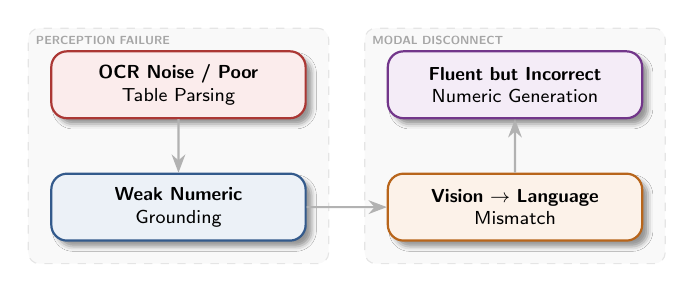
\begin{tikzpicture}[
    transform shape, 
    scale=0.85, 
    node distance=0.8cm and 1.2cm
]

    % --- LEFT COLUMN (Perception Issues) ---
    
    % 1. OCR Noise (Top Left)
    \node (step1) [stepNoise] {
        \textbf{OCR Noise / Poor} \\ 
        Table Parsing
    };

    % 2. Grounding (Bottom Left)
    \node (step2) [stepGround, below=of step1] {
        \textbf{Weak Numeric} \\ 
        Grounding
    };

    % --- RIGHT COLUMN (Integration Issues) ---
    
    % 3. Mismatch (Bottom Right - Across from Step 2)
    \node (step3) [stepMismatch, right=of step2] {
        \textbf{Vision $\to$ Language} \\ 
        Mismatch
    };

    % 4. Generation (Top Right - Above Step 3)
    \node (step4) [stepResult, above=of step3] {
        \textbf{Fluent but Incorrect} \\ 
        Numeric Generation
    };

    % --- Arrows (The U-Shape) ---
    \draw [arrow] (step1) -- (step2);  % Down
    \draw [arrow] (step2) -- (step3);  % Across
    \draw [arrow] (step3) -- (step4);  % Up

    % --- Background Grouping ---
    \begin{scope}[on background layer]
        % Group 1: Data Extraction
        \node [fit=(step1)(step2), fill=gray!5, draw=gray!20, rounded corners, dashed, inner sep=8pt] (groupL) {};
        \node [groupLabel] at (groupL.north west) {PERCEPTION FAILURE};
        
        % Group 2: Modal Integration
        \node [fit=(step3)(step4), fill=gray!5, draw=gray!20, rounded corners, dashed, inner sep=8pt] (groupR) {};
        \node [groupLabel] at (groupR.north west) {MODAL DISCONNECT};
    \end{scope}

\end{tikzpicture}
\end{document}